\documentclass[12pt,a4paper]{article}
\usepackage[utf8]{inputenc}
\usepackage[utf8]{vietnam}
\usepackage{amsmath}
\usepackage{amsfonts}
\usepackage{amssymb}
\usepackage{indentfirst}
\usepackage{graphicx}
\usepackage{subfig}
\usepackage{enumerate}
\usepackage[left=1.5cm,right=1.5cm,top=1.5cm,bottom=1.5cm]{geometry}
\graphicspath{{images/}}
\everymath{\displaystyle}

\title{\textbf{Bài tập Điều khiển quá trình \bigskip \\ Chủ đề Mô hình hóa lý thuyết}}
\author{Sưu tầm: Thi Minh Nhựt \and Email: thiminhnhut@gmail.com}
\date{Thời gian: \today}

\begin{document}

\maketitle

\section{Bài tập 1}
    \paragraph{Giả thiết}
        Cho hệ thống như hình \ref{baitap1}: Bình chứa thứ nhất có tiết diện là $A_1$ và bình chứa thứ hai có tiết diện là $A_2$. Các lưu lượng ra $Q_b$ và $Q_c$ được xác định như sau: $Q_b = C_{db}a_b\sqrt{2g(H_1 - H_2)}$ và $Q_c = C_{dc}a_c\sqrt{2gH_2}$
        \begin{figure}[htp]
            \begin{center}
                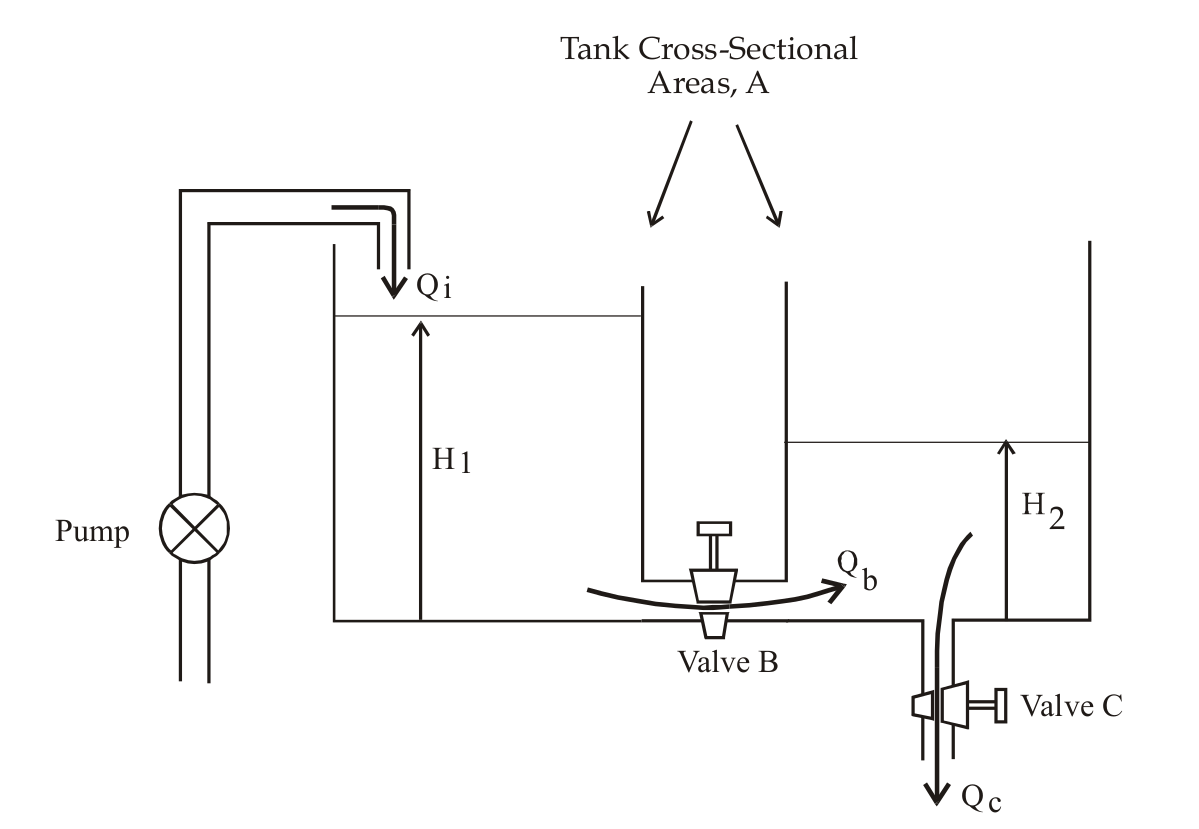
\includegraphics[scale=.3]{bai1}
            \end{center}
            \caption{Hệ thống 2 bình chứa} \label{baitap1}
        \end{figure}

    \paragraph{Yêu cầu}
        \begin{enumerate}[a.]
            \item Xác định các biến vào, biến ra, biến điều khiển, biến cần điều khiển và biến nhiễu.
            \item Viết phương trình mô tả quan hệ giữa các biến.
            \item Tuyến tính hóa mô hình tại điểm làm việc cân bằng.
            \item Tìm hàm truyền $G(s) = \dfrac{H_2(s)}{Q_i(s)}$
        \end{enumerate}

    \paragraph{Bài giải}
        \begin{enumerate}[\it a.]
            \item \textit{Xác định các biến vào, biến ra, biến điều khiển, biến cần điều khiển và biến nhiễu.}
                \begin{itemize}
                    \item Biến vào: $Q_i, Q_b, Q_c$.
                    \item Biến ra: $H_1, H_2$.
                    \item Biến điều khiển: $Q_b, Q_c$.
                    \item Biến cần điều khiển: $H_1, H_2$.
                    \item Biến nhiễu: $Q_i$.
                \end{itemize}

            \item \textit{Viết phương trình mô tả quan hệ giữa các biến.}
                \begin{itemize}
                    \item Phương trình cho bình chứa 1:
                        \begin{itemize}
                            \item Bình chứa 1:
                                \begin{align} \label{eq:talk-1}
                                    \frac{dV_1}{dt} = Q_i - Q_b \Longleftrightarrow \dfrac{d \left({A_1 H_1}\right)}{dt} = Q_i - Q_b \Longleftrightarrow \dfrac{d H_1}{dt} = \dfrac{1}{A_1} \left({Q_i - Q_b}\right)
                                \end{align}

                            \item Thay $Q_b = C_{db}a_b\sqrt{2g(H_1 - H_2)}$ vào (\ref{eq:talk-1}), ta có:
                                \begin{align} \label{eq:talk-1-2}
                                    \dfrac{dH_1}{dt} = \dfrac{1}{A_1} \left({Q_i - Q_b}\right) = \dfrac{1}{A_1} \left[{Q_i - C_{db}a_b\sqrt{2g(H_1 - H_2)}}\right]
                                \end{align}
                        \end{itemize}

                    \item Phương trình cho bình chứa 2:
                        \begin{itemize}
                            \item Bình chứa 2:
                                \begin{align} \label{eq:talk-2}
                                    \dfrac{dV_2}{dt} = Q_b - Q_c \Longleftrightarrow \dfrac{d \left({A_2 H_2}\right)}{dt} = Q_b - Q_c \Longleftrightarrow \dfrac{d H_2}{dt} = \dfrac{1}{A_2} \left({Q_b - Q_c}\right)
                                \end{align}

                            \item Thay $Q_b = C_{db}a_b\sqrt{2g(H_1 - H_2)}$ và $Q_c = C_{dc}a_c\sqrt{2gH_2}$ vào (\ref{eq:talk-2}), ta có:
                                \begin{align} \label{eq:talk-2-2}
                                    \dfrac{dH_2}{dt} = \dfrac{1}{A_2} \left({Q_b - Q_c}\right) = \dfrac{1}{A_2} \left[{C_{db}a_b\sqrt{2g(H_1 - H_2)} - C_{dc}a_c\sqrt{2gH_2}}\right]
                                \end{align}
                        \end{itemize}

                    \item Kết luận, hệ phương trình mô tả quá trình:
                        \begin{align}
                            \left\{
                            \begin{array}{l}
                                \dfrac{dH_1}{dt} = \dfrac{1}{A_1} \left[{Q_i - C_{db}a_b\sqrt{2g(H_1 - H_2)}}\right]\\ [.5cm]
                                \dfrac{dH_2}{dt} = \dfrac{1}{A_2} \left[{C_{db}a_b\sqrt{2g(H_1 - H_2)} - C_{dc}a_c\sqrt{2gH_2}}\right]
                            \end{array}
                            \right.
                        \end{align}
                \end{itemize}

            \item \textit{Tuyến tính hóa mô hình tại điểm làm việc cân bằng.}
                \begin{itemize}
                    \item Gọi $\left({ \overline{Q_i}, \overline{H_1}, \overline{H_2}}\right)$ là điểm làm việc cân bằng của hệ thống gồm 2 bình chứa.

                    \item Gọi $Q_i = \overline{Q_i} + \Delta Q_i, H_1 = \overline{H_1} + \Delta H_1, H_2 = \overline{H_2} + \Delta H_2$.

                    \item Đặt $f\left({Q_i, H_1, H_2}\right) = \dot{H_1} = \dfrac{1}{A_1} \left[{Q_i - C_{db}a_b\sqrt{2g(H_1 - H_2)}}\right]$
                        \begin{itemize}
                            \item Tại điểm làm việc cân bằng $\left({ \overline{Q_i}, \overline{H_1}, \overline{H_2}}\right)$ thì
                                \begin{align}
                                    f\left({ \overline{Q_i}, \overline{H_1}, \overline{H_2}}\right) = 0 \Longleftrightarrow \dfrac{1}{A_1} \left[{\overline{Q_i} - C_{db}a_b\sqrt{2g(\overline{H_1} - \overline{H_2})}}\right] = 0
                                \end{align}

                            \item Khai triển Taylor cho $f\left({Q_i, H_1, H_2}\right) = \dot{H_1} = \dfrac{1}{A_1} \left[{Q_i - C_{db}a_b\sqrt{2g(H_1 - H_2)}}\right]$, ta có:
                                \begin{align}
                                    \dot{H_1} = \Delta H_1 & = f\left({\overline{Q_i} + \Delta Q_i, \overline{H_1} + \Delta H_1, \overline{H_2} + \Delta H_2}\right) \\
                                    & \approx \underbrace{f\left({ \overline{Q_i}, \overline{H_1}, \overline{H_2}}\right)}_{0} + \left.\dfrac{\partial f}{\partial Q_i}\right|_{ \left({ \overline{Q_i}, \overline{H_1}, \overline{H_2}}\right)} \Delta Q_i + \left.\dfrac{\partial f}{\partial H_1}\right|_{ \left({ \overline{Q_i}, \overline{H_1}, \overline{H_2}}\right)} \Delta H_1\\
                                    & \approx \dfrac{1}{A_1} \left[{\Delta Q_i - \dfrac{2gC_{db}a_b}{2\sqrt{2g(\overline{H_1} - \overline{H_2})}} \Delta H_1}\right]\\
                                    & \approx \dfrac{1}{A_1} \left[{\Delta Q_i - \dfrac{gC_{db}a_b}{\sqrt{2g(\overline{H_1} - \overline{H_2})}} \Delta H_1}\right]
                                \end{align}

                            \item Thay $\Delta Q_i = Q_i$ và $\Delta H_1 = H_1$, ta có:
                                \begin{align}
                                    \dfrac{d H_1}{dt} = \dfrac{1}{A_1} \left[{Q_i - \dfrac{gC_{db}a_b}{\sqrt{2g(\overline{H_1} - \overline{H_2})}} H_1}\right]
                                \end{align}
                        \end{itemize}

                    \item Đặt $g\left({Q_i, H_1, H_2}\right) = \dot{H_2} = \dfrac{1}{A_2} \left[{C_{db}a_b\sqrt{2g(H_1 - H_2)} - C_{dc}a_c\sqrt{2gH_2}}\right]$
                        \begin{itemize}
                            \item Tại điểm làm việc cân bằng $\left({ \overline{Q_i}, \overline{H_1}, \overline{H_2}}\right)$ thì:
                                \begin{align}
                                    g\left({ \overline{Q_i}, \overline{H_1}, \overline{H_2}}\right) = 0 \Longleftrightarrow \dfrac{1}{A_2} \left[{C_{db}a_b\sqrt{2g(\overline{H_1} - \overline{H_2})} - C_{dc}a_c\sqrt{2g \overline{H2}}}\right] = 0
                                \end{align}

                            \item Khai triển Taylor cho $g\left({Q_i, H_1, H_2}\right) = \dot{H_2} = \dfrac{1}{A_2} \left[{C_{db}a_b\sqrt{2g(H_1 - H_2)} - C_{dc}a_c\sqrt{2gH_2}}\right]$, ta có:
                                \begin{align}
                                    \dot{H_2} = \Delta H_2 & = g\left({\overline{Q_i} + \Delta Q_i, \overline{H_1} + \Delta H_1, \overline{H_2} + \Delta H_2}\right) \\
                                    & \approx \underbrace{g\left({ \overline{Q_i}, \overline{H_1}, \overline{H_2}}\right)}_{0} + \left.\dfrac{\partial g}{\partial H_1}\right|_{ \left({ \overline{Q_i}, \overline{H_1}, \overline{H_2}}\right)} \Delta H_1 + \left.\dfrac{\partial g}{\partial H_2}\right|_{ \left({ \overline{Q_i}, \overline{H_1}, \overline{H_2}}\right)} \Delta H_2\\
                                    & \approx \dfrac{1}{A_2} \left[{\dfrac{2g C_{db}a_b}{2 \sqrt{2g(\overline{H_1} - \overline{H_2})}} \Delta H_1 + \dfrac{-2g C_{db}a_b}{2 \sqrt{2g(\overline{H_1} - \overline{H_2})}} \Delta H_2 - \dfrac{2g C_{dc}a_c}{2 \sqrt{2g\overline{H_2}}} \Delta H_2 }\right]\\
                                    & \approx \dfrac{1}{A_2} \left[{\dfrac{g C_{db}a_b}{\sqrt{2g(\overline{H_1} - \overline{H_2})}} \Delta H_1 - \dfrac{g C_{db}a_b}{ \sqrt{2g(\overline{H_1} - \overline{H_2})}} \Delta H_2 - \dfrac{g C_{dc}a_c}{\sqrt{2g\overline{H_2}}} \Delta H_2 }\right]
                                \end{align}

                            \item Thay $\Delta H_1= H_1$ và $\Delta H_2 = H_2$, ta có:
                                \begin{align}
                                    \dfrac{d H_2}{dt} = \dfrac{1}{A_2} \left[{\dfrac{g C_{db}a_b}{\sqrt{2g(\overline{H_1} - \overline{H_2})}} H_1 - \dfrac{g C_{db}a_b}{ \sqrt{2g(\overline{H_1} - \overline{H_2})}} H_2 - \dfrac{g C_{dc}a_c}{\sqrt{2g\overline{H_2}}} H_2 }\right]
                                \end{align}
                        \end{itemize}

                    \item Kết luận, phương trình tuyến tính hóa của mô hình tại điểm làm việc cân bằng $\left({ \overline{Q_i}, \overline{H_1}, \overline{H_2}}\right)$:
                        \begin{align}
                            \left\{
                            \begin{array}{l}
                                \dfrac{dH_1}{dt} = \dfrac{1}{A_1} \left[{Q_i - \dfrac{gC_{db}a_b}{\sqrt{2g(\overline{H_1} - \overline{H_2})}} H_1}\right]\\ [.5cm]
                                \dfrac{dH_2}{dt} = \dfrac{1}{A_2} \left[{\dfrac{g C_{db}a_b}{\sqrt{2g(\overline{H_1} - \overline{H_2})}} H_1 - \dfrac{g C_{db}a_b}{ \sqrt{2g(\overline{H_1} - \overline{H_2})}} H_2 - \dfrac{g C_{dc}a_c}{\sqrt{2g\overline{H_2}}} H_2 }\right]
                            \end{array}
                            \right.
                        \end{align}
                \end{itemize}

            \item \textit{Tìm hàm truyền $G(s) = \dfrac{H_2(s)}{Q_i(s)}$}
                \begin{itemize}
                    \item Ta có: $\dfrac{dH_1}{dt} = \dfrac{1}{A_1} \left[{Q_i - \dfrac{gC_{db}a_b}{\sqrt{2g(\overline{H_1} - \overline{H_2})}} H_1}\right]$, thực hiện biến đổi Laplace 2 vế của phương trình ta có:
                        \begin{align}
                            & s H_1(s) = \dfrac{1}{A_1} \left[{Q_i(s) - \dfrac{gC_{db}a_b}{\sqrt{2g(\overline{H_1} - \overline{H_2})}} H_1(s)}\right]\\
                            \Longleftrightarrow & s A_1 H_1(s) + \dfrac{gC_{db}a_b}{\sqrt{2g(\overline{H_1} - \overline{H_2})}} H_1(s) = Q_i(s)\\
                            \Longleftrightarrow & \left[{s A_1 + \dfrac{gC_{db}a_b}{\sqrt{2g(\overline{H_1} - \overline{H_2})}} }\right] H_1(s) = Q_i(s) \\
                            \Longleftrightarrow & H_1(s) = \frac{Q_i(s)}{s A_1 + \dfrac{gC_{db}a_b}{\sqrt{2g(\overline{H_1} - \overline{H_2})}}}
                        \end{align}
                    \item Ta có: $\dfrac{dH_2}{dt} = \dfrac{1}{A_2} \left[{\dfrac{g C_{db}a_b}{\sqrt{2g(\overline{H_1} - \overline{H_2})}} H_1 - \dfrac{g C_{db}a_b}{ \sqrt{2g(\overline{H_1} - \overline{H_2})}} H_2 - \dfrac{g C_{dc}a_c}{\sqrt{2g\overline{H_2}}} H_2 }\right]$, thực hiện biến đổi Laplace 2 vế của phương trình ta có:
                        \begin{align}
                            & s H_2(s) = \dfrac{1}{A_2} \left[{\dfrac{g C_{db}a_b}{\sqrt{2g(\overline{H_1} - \overline{H_2})}} H_1(s) - \dfrac{g C_{db}a_b}{ \sqrt{2g(\overline{H_1} - \overline{H_2})}} H_2 (s) - \dfrac{g C_{dc}a_c}{\sqrt{2g\overline{H_2}}} H_2 (s) }\right] \\
                            \Longleftrightarrow & s A_2 H_2(s) + \dfrac{g C_{db}a_b}{ \sqrt{2g(\overline{H_1} - \overline{H_2})}} H_2 (s) + \dfrac{g C_{dc}a_c}{\sqrt{2g\overline{H_2}}} H_2 (s) = \dfrac{g C_{db}a_b}{\sqrt{2g(\overline{H_1} - \overline{H_2})}} H_1(s) \\
                            \Longleftrightarrow & \left[{s A_2 + \dfrac{g C_{db}a_b}{ \sqrt{2g(\overline{H_1} - \overline{H_2})}} + \dfrac{g C_{dc}a_c}{\sqrt{2g\overline{H_2}}} }\right] H_2 (s) = \dfrac{g C_{db}a_b}{\sqrt{2g(\overline{H_1} - \overline{H_2})}} H_1(s)\\
                            \Longleftrightarrow & \left[{s A_2 + \dfrac{g C_{db}a_b}{ \sqrt{2g(\overline{H_1} - \overline{H_2})}} + \dfrac{g C_{dc}a_c}{\sqrt{2g\overline{H_2}}} }\right] H_2 (s) = \dfrac{g C_{db}a_b Q_i(s)}{\sqrt{2g(\overline{H_1} - \overline{H_2})} \left[{s A_1 + \dfrac{gC_{db}a_b}{\sqrt{2g(\overline{H_1} - \overline{H_2})}}}\right]} \\
                            \Longleftrightarrow & \left[{s A_2 + \dfrac{g C_{db}a_b}{ \sqrt{2g(\overline{H_1} - \overline{H_2})}} + \dfrac{g C_{dc}a_c}{\sqrt{2g\overline{H_2}}} }\right] H_2 (s) = \dfrac{g C_{db}a_b Q_i(s)}{s A_1 \sqrt{2g(\overline{H_1} - \overline{H_2})} + gC_{db}a_b} \\
                            \Longleftrightarrow & \dfrac{H_2(s)}{Q_i(s)} = \dfrac{g C_{db}a_b}{\left[{s A_2 + \dfrac{g C_{db}a_b}{ \sqrt{2g(\overline{H_1} - \overline{H_2})}} + \dfrac{g C_{dc}a_c}{\sqrt{2g\overline{H_2}}} }\right]  \left[{ s A_1 \sqrt{2g(\overline{H_1} - \overline{H_2})} + gC_{db}a_b }\right]}
                        \end{align}

                    \item Kết luận: $G(s) = \dfrac{H_2(s)}{Q_i(s)} = \dfrac{g C_{db}a_b}{\left[{s A_2 + \dfrac{g C_{db}a_b}{ \sqrt{2g(\overline{H_1} - \overline{H_2})}} + \dfrac{g C_{dc}a_c}
                    {\sqrt{2g\overline{H_2}}} }\right]  \left[{ s A_1 \sqrt{2g(\overline{H_1} - \overline{H_2})} + gC_{db}a_b }\right]}$
                \end{itemize}
        \end{enumerate}


\section{Bài tập 2}
    \paragraph{Giả thiết}
    Cho hệ thống như hình \ref{baitap2}:  Các lưu lượng ra $q_1$ và $q_0$ được xác định như sau: $q_1 = \dfrac{h_1 - h_2}{R_1}$ và $q_0 = \dfrac{h_2}{R_2}$
    \begin{figure}[htp]
        \begin{center}
            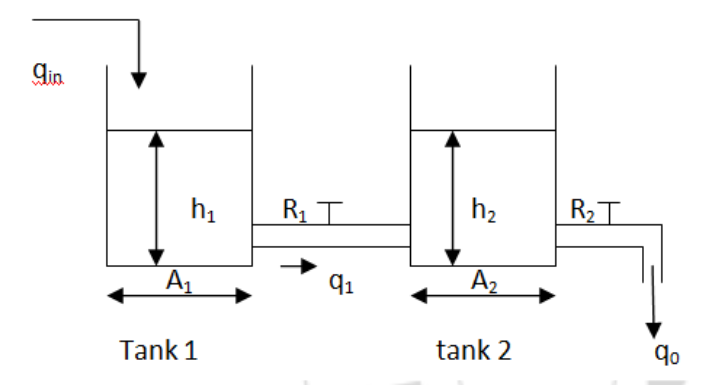
\includegraphics[scale=.5]{bai2}
        \end{center}
        \caption{Hệ thống 2 bình chứa} \label{baitap2}
    \end{figure}

    \paragraph{Yêu cầu}
        \begin{enumerate}[a.]
            \item Xác định các biến vào, biến ra, biến điều khiển, biến cần điều khiển và biến nhiễu.
            \item Viết phương trình mô tả quan hệ giữa các biến.
            \item Tuyến tính hóa mô hình tại điểm làm việc cân bằng.
            \item Tìm hàm truyền $G(s) = \dfrac{H_2(s)}{Q_{in}(s)}$
        \end{enumerate}
\end{document}
